%!TEX program = xelatex
\documentclass[11pt]{article}

\usepackage[x11names]{xcolor} % needed to declare before tikz
\usepackage{amsmath,  latexsym, amssymb, url, amssymb, pgfplots, amsthm, mathtools, setspace, commath, tikz, verbatim, array, enumitem, bbding, bigints, fontspec, xunicode, xltxtra, geometry, algorithm, algpseudocode, graphicx,listings,lipsum,tabto,tcolorbox,sectsty,booktabs,siunitx,caption, float}
\usepackage[version=4]{mhchem}
\usepackage[utf8]{inputenc}

\NumTabs{6}

\defaultfontfeatures{Mapping=tex-text} 

\setmainfont{Charter} 

\newfontfamily\Codefont{Courier}  %{GillSans} %{AmericanTypewriter}

\definecolor{gry}{rgb}{.95,.95,.95}

\lstset{language=C++,
                moredelim=[is][\color{Green3}\Codefont]{<}{>},
                basicstyle=\small\Codefont,
                identifierstyle=\Codefont,
                directivestyle=\color{Coral1}\Codefont,
                keywordstyle=\color{DeepPink2}\Codefont,
                stringstyle=\color{SeaGreen4}\Codefont,
                commentstyle=\color{Snow4}\Codefont,
                emphstyle=\color{DeepSkyBlue3}\Codefont,
                emph={double,int,float,void,long},
                showspaces=false,
                %keywordstyle=[2]\color{Violet},
                keywords=[2]{*,1,2,3,4,5,6,7,8,9,0},
                keywordstyle=[2]\color{blue},
                showstringspaces=false,
                morecomment=[l][\color{orange}]{\#}}
\lstset{literate=%
    *{0}{{{\color{DarkOrchid3}0}}}1
    {1}{{{\color{DarkOrchid3}1}}}1
    {2}{{{\color{DarkOrchid3}2}}}1
    {3}{{{\color{DarkOrchid3}3}}}1
    {4}{{{\color{DarkOrchid3}4}}}1
    {5}{{{\color{DarkOrchid3}5}}}1
    {6}{{{\color{DarkOrchid3}6}}}1
    {7}{{{\color{DarkOrchid3}7}}}1
    {8}{{{\color{DarkOrchid3}8}}}1
    {9}{{{\color{DarkOrchid3}9}}}1
    {.0}{{{\color{DarkOrchid3}.0}}}2
    {.1}{{{\color{DarkOrchid3}.1}}}2
    {.2}{{{\color{DarkOrchid3}.2}}}2
    {.3}{{{\color{DarkOrchid3}.3}}}2
    {.4}{{{\color{DarkOrchid3}.4}}}2
    {.5}{{{\color{DarkOrchid3}.5}}}2
    {.6}{{{\color{DarkOrchid3}.6}}}2
    {.7}{{{\color{DarkOrchid3}.7}}}2
    {.8}{{{\color{DarkOrchid3}.8}}}2
    {.9}{{{\color{DarkOrchid3}.9}}}2
}
\lstset{alsolanguage=[90]Fortran}
\lstset{alsolanguage=python}
\lstset{backgroundcolor=\color{gry}}
\lstset{frame=single}
\lstset{
    numbers=left,
    numberstyle=\Codefont,
    title=\lstname,
    tabsize=4,
}
\geometry{margin=1in}
\geometry{letterpaper} % or letterpaper (US) or a5paper or....
\usepackage[parfill]{parskip} % Activated to begin paragraphs with an empty line rather than an indent

\title{PHY 480 - Computational Physics \\ Project 2: Schr\"{o}dinger's Equation for 2 electrons in a 3D Well}
\author{Thomas Bolden}
\date{March 4, 2016}

\usepackage{hyperref}
\hypersetup{
    colorlinks=true,
    linkcolor=darkgray,
    filecolor=magenta,      
    urlcolor=Aquamarine3, %DarkSlateGray4,
}

\setcounter{secnumdepth}{0} % deactivate for section numbers
%\sectionfont{\fontsize{12}{15}\selectfont} % Activate for same font size sections
\subsectionfont{\fontsize{15}{15}\selectfont}
\newenvironment{amatrix}[1]{%
  \left[\begin{array}{@{}*{#1}{c}|c@{}}
}{%
  \end{array}\right]
}

\setmainfont{Charter}

\begin{document}

\maketitle

\thispagestyle{empty}

\centerline{Github Repository at \href{https://github.com/ThomasBolden/PHY-480-Spring-2016}{https://github.com/ThomasBolden/PHY-480-Spring-2016}}

\begin{abstract}

    In this project, a solution was found to the two-electron Schr\"{o}dinger equation in three-dimensions. This was done by diagonalizing an $n$ by $n$ matrix to find the eigenfunctions and eigenvectors of the three lowest energy states. Computation time to determine the eigenvalues was compared between a brute-force implimentation of Jacobi's algorithm and the Armadillo library. For large $n$, the Armadillo library is orders of magnitude faster. Using the Armadillo {\em eig\_sys} function, the wavefunctions of the lowest three energies are compared while varying the strength of the harmonic oscillator potential.

\end{abstract}

\vfill

\tableofcontents

\vspace{3cm}

\pagebreak

\subsection{Introduction}

    In physics, there is a known solution to Schr\"{o}dinger's equation for a single electron in a spherically symmetric three-dimensional well. However, this equation becomes more complicated when another elctron is added. In addition to the energy term, there are Coulombic interactions between the electrons that must be accounted for. 

    For one electron, the radial part of the Schr\"{o}dinger equation reads
    \[ -\dfrac{\hbar^2}{2m} \left( \dfrac{1}{r^2} \dfrac{d}{dr}r^2\dfrac{d}{dr} - \dfrac{\ell (\ell -1)}{r^2} \right) R(r) + V(r) R(r) = E R(r) \;\; , \;\; V(r) = \dfrac{m\omega^2 r^2}{2}. \]
    In this case, the potential function for the harmonic oscillator is $V(r) = \dfrac{m\omega^2}{2}$, and $E$ is the 3D energy. With th quantum numbers $n$ and $l$, the energies are given by
    \[ E_{nl} = \hbar \omega \left( 2n+l+\dfrac{3}{2} \right). \]

    If we are to solve this computationally, it is helpful to introduce a dimensionless variable $\rho = 1/\alpha$, with $\alpha$ is the length constant. 
    \[ -\dfrac{\hbar^2}{2m\alpha^2} \dfrac{d^2}{d\rho^2} u(\rho) + \left( V(\rho) + \dfrac{l(l+1)}{\rho^2} \dfrac{\hbar^2}{2m\alpha^2} \right) u(\rho) = Eu(\rho) \]
    If we neglect angular momentum by setting $l=0$, and making $\omega = \alpha \rho$, we get
    \[ -\dfrac{\hbar^2}{2m\alpha^2} \dfrac{d^2}{d\rho^2} u(\rho) + \dfrac{k}{2} \alpha^2 \rho^2 u(\rho) = Eu(\rho) \]
    If both sides of thie equation are multiplied by $\dfrac{2m\alpha^2}{\hbar^2}$ and fixing $\alpha = \left( \dfrac{\hbar^2}{mk} \right)^{1/4}$ the equation becomes
    \[ -\dfrac{d^2}{d\rho^2} u(\rho)+ \rho^2 u(\rho) = \lambda u(\rho). \]
    Discrete energy eigenvalues are given by
    \[ \lambda = \dfrac{2m\alpha^2}{\hbar^2}. \]
    The first three eigenvalues are the $\lambda_0 = 3$, $\lambda_1 = 7$, $\lambda_2 = 11$. 

    In order to solve this, the standard approximation of the second derivatve with step length $h$,
    \[ u\prime \prime = \dfrac{u(\rho+h)-2u(\rho)+u(\rho-h)}{h^2} + O(h^2) , \]
    will be used. The finial tridiagonal matrix is then

    \[
    \left( \begin{array}{ccccccc} \frac{2}{h^2}+V_1 & -\frac{1}{h^2} & 0   & 0    & \dots  &0     & 0 \\
    -\frac{1}{h^2} & \frac{2}{h^2}+V_2 & -\frac{1}{h^2} & 0    & \dots  &0     &0 \\
    0   & -\frac{1}{h^2} & \frac{2}{h^2}+V_3 & -\frac{1}{h^2}  &0       &\dots & 0\\
    \dots  & \dots & \dots & \dots  &\dots      &\dots & \dots\\
    0   & \dots & \dots & \dots  &\dots       &\frac{2}{h^2}+V_{n_{\mathrm{steps}}-2} & -\frac{1}{h^2}\\
    0   & \dots & \dots & \dots  &\dots       &-\frac{1}{h^2} & \frac{2}{h^2}+V_{n_{\mathrm{steps}}-1}
    \end{array} \right)  .
    \]

    In this project, I explore and compare various ways to solve the two-electron Schr\"{o}dinger equation. In the following section, the methods used to write and impliment the Jacobi rotation code are discussed. In the Results section, I present the data I have found. I discuss it in some detail, but most of the analysis is saved for the Conclusions section. Finally, the Code section is a collection of the code used to produce the results.

\subsection{Methods}

    %\subsubsection{Jacobi's Rotation Algorithm}

        The general algorithm for Jacobi's rotation is as follows:

         Update !! !!!!!!!!!!!!!!!!!!!!!!!!!!!!
        \begin{algorithm}[H]
        \caption{Jacobi Rotation}
        \label{Jacobi Rotation}
        \begin{algorithmic}[1]
        \Procedure Jacobi Rotation
        \State $n \times n$ matrix A
        \Function MaxOffDiagonal
        \EndFunction
        \EndProcedure
        \end{algorithmic}
        \end{algorithm}

        When implimenting this algorithm, it is important to choose the smaller magnitude solution to $t = -\tau \pm \sqrt{1+\tau^2}$. To get a sense of why, it is best to use the equation
        \[ \abs{\abs{\mathbf{B} - \mathbf{A}}}_F^2 = 4 (1-c) \sum_{i=1,i\neq k,l}^n (a_{ik}^2 + a_{il}^2) + \dfrac{2a_{kl}^2}{c^2}. \] 
        This equation, with $c=\dfrac{1}{1+t^2}$, gives the difference between matrices $\mathbf{A}$ and $\mathbf{B}$. Since we want to minimize this difference, it becomes clear that we want to take a value of $c$ to be as close to 1 as possible. Doing this will make the $(1-c)$ term go to zero. Since we want a value of $c$ that is close to one, the $t$ value chosen must be as small as possible. This is because of the way $c$ is defined above. With small $t$, the denominator approaches 1, allowing $c$ to also approach 1.

        %This is because in the equation for cosine, 

\subsection{Results}

    %\subsubsection{Eigenvalue Computation Time Comparison} %vs the Armadillo Library} % ?

        %The Armadillo library has a function called {\em eig\_sym} which computes the eigenvalues of a system. The computation time for this function was compared to the computation time using Jacobi's algorithm. The results are displayed below in Table 1. They are then graphed in Figure 1.

    When the dimensionality of the matrix is changed, the  dimensionless variable $\rho$ needed to accurately determine the lowest three eigenvectors also changes. The data is graphed in Table 1, and graphed in Figure 1.

        %\table
    \begin{table}[H]
    \caption{Checking $\rho$ Dependency for Various Matrix Dimensionality}
    \[
    \begin{array}{cc}
    \toprule \midrule
     \text{Minimum } \rho_\text{max} & \text{Matrix Dimensions } n  \\ \midrule
    5 & 200 \\ \midrule
    6 & 250 \\ \midrule
    7 & 300 \\ \midrule
    8 & 350 \\ \midrule
    9 & 400 \\ \midrule
    10 & 450 \\ \midrule
    \bottomrule
    \end{array}
    \]
    \end{table}

    %\figure graph using RhoDependency.py

    % as you can see with 50 step size in n, the trend is perfectly linear

    \begin{figure}[H] \begin{center}
    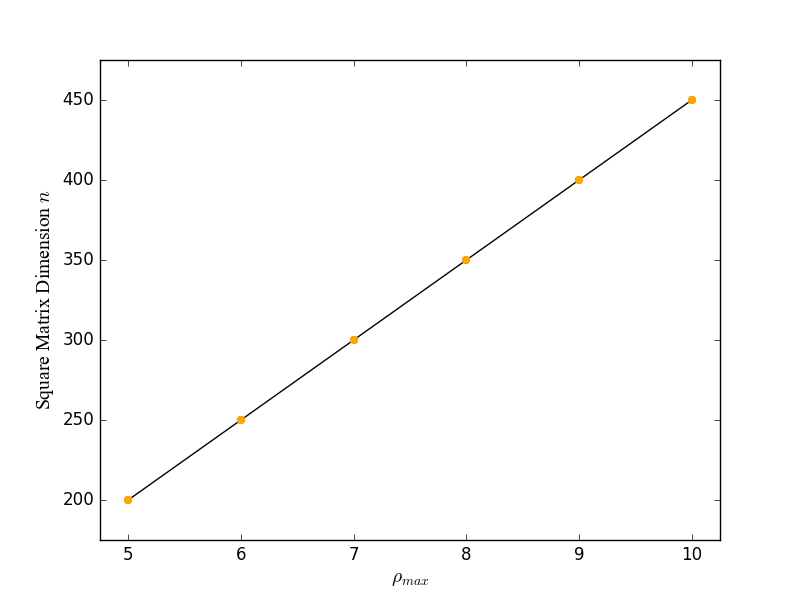
\includegraphics[width=0.8\textwidth]{../Code/RhoDepend.png}
    \end{center} \caption{Value of $\rho$ Required for Accurate Eigenvalues} \end{figure}

    With a step size of 50 for the matrix dimensinality, the relationship between $\rho$ and $n$ is perfectly linear.

    Using this fact, one can test the number of similarity transformations required to effectively diagonalize the matrices. Implimentation of \texttt{EigensolverTests.cpp} gives these results. Here, the tolerance for a nondiagonal matrix element was set to $ \epsilon = 1 \times 10^{-10}$. The number of transformations required to diagonalize a square matrix of dimension $n$ are listed in Table 2. The computation times are also compared between Jacobi's algorithm and Armadillo's library.

    %\begin{algorithm}
    %\caption{Gaussian Elimination}
    %\label{Gaussian Elimination}
    %\begin{algorithmic}[1]
    %\Function{GaussElim}{A}
    %\For{$k=1$ to  $n-1$}
    %\For{$i=k+1$ to $n$}
    %\State $a_{ik} = \frac{a_{ik}}{a_{kk}}$
    %\For{$j=k+1$ to $n+1$}
    %\State $a_{ij}=a_{ij}-a_{ik}\times a_{kj}$
    %\EndFor
    %\EndFor
    %\EndFor
    %\EndFunction
    %\end{algorithmic}
    %\end{algorithm}

    \begin{table}[H]
    \caption{Comparing Jacobi's Algorithm to Armadillo Using $\rho = 5.0$}
    \[
    \begin{array}{c|cccc}
    \toprule \midrule
    \text{Dimensionality $n$} & \text{Eigenvalues} & t_\text{Armadillo} \text{ (s)} & t_\text{Jacobi} \text{ (s)} & \text{Transformations} \\ \midrule
     50   &  (2.99687, 6.98434, 10.9619)  &   0.000617    &    0.08572    &     4139 \\ \midrule
    100   &  (2.99922, 6.99609, 10.9907)  &    0.003777  &        1.15983  &      17293 \\ \midrule
    150  &   (2.99965, 6.99827, 10.9960)  &    0.007561    &      5.89020    &    39377 \\ \midrule
     200   &  (2.99980, 6.99903, 10.9978) &      0.012636       &  18.5741  &      70538 \\ \midrule
    250  &   (2.99988, 6.99938, 10.9987)   &    0.019315       &   49.3644     &  110646 \\ \midrule
    300  &   (2.99991, 6.99957, 10.9991)    &   0.032661  &        110.025   &    160133 \\ \midrule
    350  &   (2.99994, 6.99968, 10.9994)    &   0.061280     &     248.396      & 218405 \\ \midrule
    400  &   (2.99995, 6.99976, 10.9996)    &   0.086203     &     430.594    &   284916 \\ \midrule
    450  &   (2.99996, 6.99981, 10.9997)    &   0.094821  &        901.509   &    361794 \\ \midrule
    500  &   (2.99997, 6.99985, 10.9998)   &     0.123586   &       1394.52     &  447415 \\ \midrule
    \bottomrule
    \end{array}
    \] 
    %\caption*{The program comparing these two methods was written in C++ 14. Jacobi's brute force algorithm ise used to diagonalize a matrix of size $n$. Armadillo's function {\em eig\_sym} was used to find eigenvectors. The eigenvalues presented are the lowest three.}
    \end{table}

    From this data, the number of transformations based on the dimensionality of the matrix was graphed. The curve was fit quadratically using {\em polyfit} from the numerical python library. The graph and its equation are shown in Figure 2.

    \begin{figure}[H] \begin{center}
    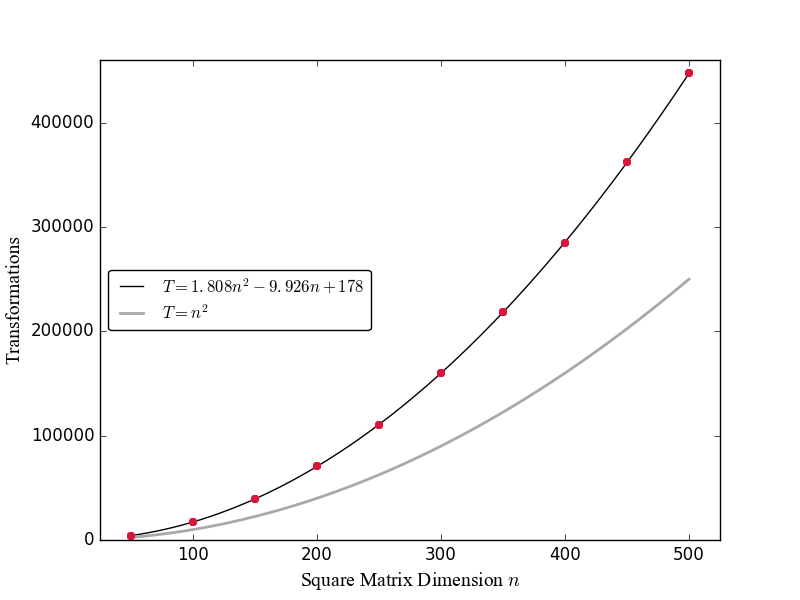
\includegraphics[width=0.6\textwidth]{../Code/TvsN.png}
    \end{center} \caption{Tansformations Increasing with Dimensionality} \end{figure}

    The next task was to plot the two-electron wavefunctions as a function of the relative coordinate $\rho$ and varying values of $\omega_r$. In the figures that follow, the two-electron wavefunctions are plotted as probability distributions. Four values for $\omega_r$ were used and compared. They are: $\omega_r = \{ 0.01 , 0.50 , 1.00 , 5.00 \}$. The wavefunctions assumed the electron in the ground state, with $l = 0$. The first three eigenvectors graphed were found using Armadillo's {\em eig\_sys} function.

    \begin{figure}[H] \begin{center}
    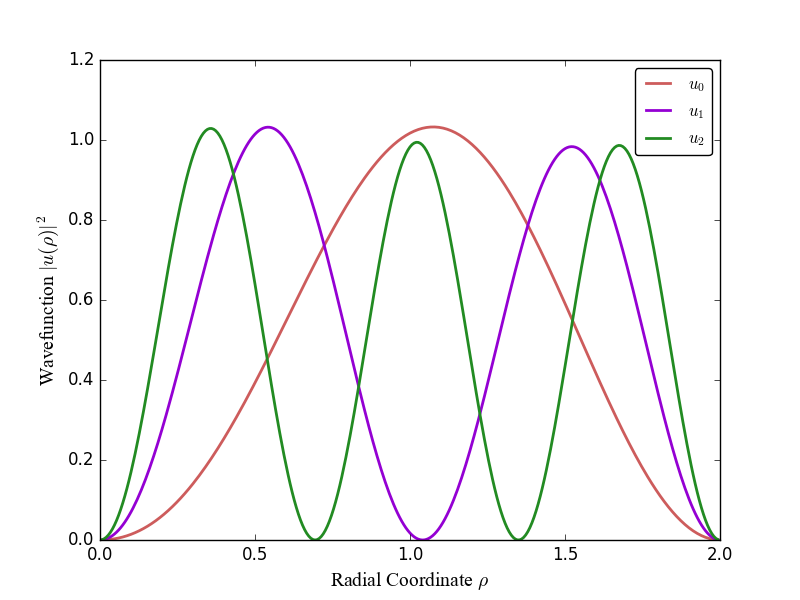
\includegraphics[width=0.8\textwidth]{../Code/WavefunctionOmega0p01.png}
    \end{center} \caption{Wavefunction with $\omega_r = 0.01$} \end{figure}

    \begin{figure}[H] \begin{center}
    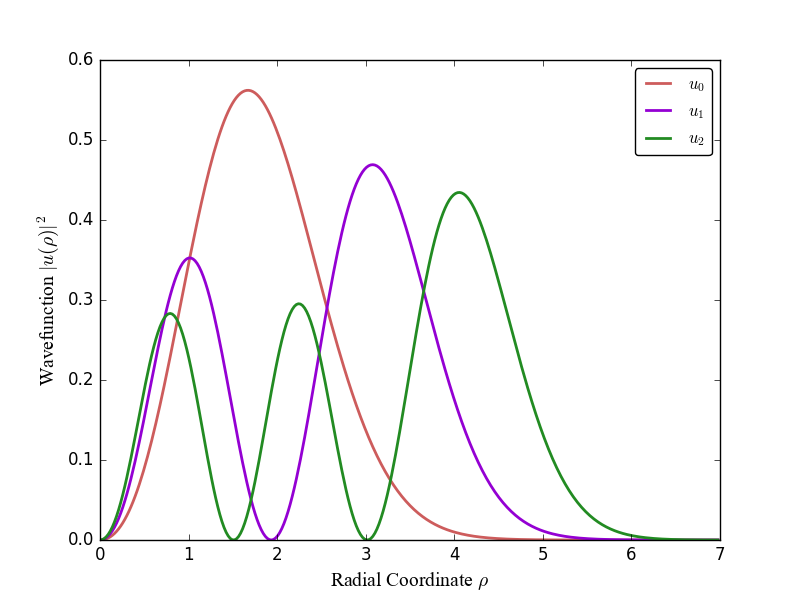
\includegraphics[width=0.8\textwidth]{../Code/WavefunctionOmega0p50.png}
    \end{center} 
    \caption{Wavefunction with $\omega_r = 0.50$} \end{figure}

    \begin{figure}[H] \begin{center}
    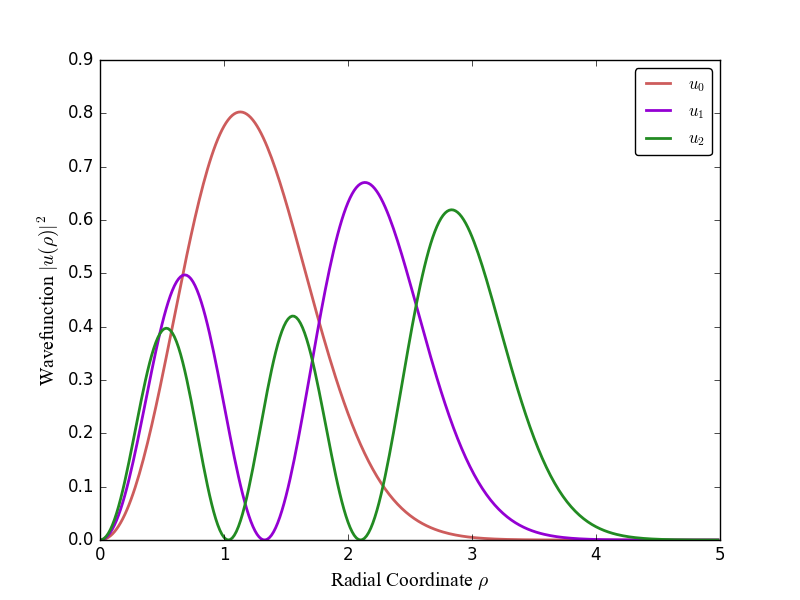
\includegraphics[width=0.8\textwidth]{../Code/WavefunctionOmega1.png}
    \end{center} \caption{Wavefunction with $\omega_r = 1.00$} \end{figure}

    \begin{figure}[H] \begin{center}
    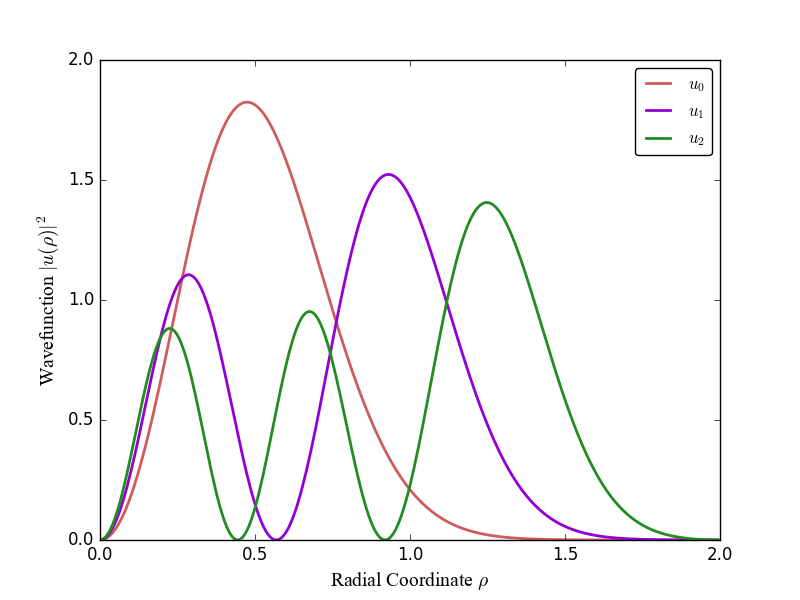
\includegraphics[width=0.8\textwidth]{../Code/WavefunctionOmega5.png}
    \end{center} \caption{Wavefunction with $\omega_r = 5.00$} \end{figure}

\subsection{Conclusions}

    Jacobi's method for diagonalizing matrices was found to be orders of magnitude slower than the Armadillo library's {\em eig\_sys} function. This means that, while useful and simple to impliment, Jacobi's method is only practical for small matrices.

\subsection{Code}

    \lstinputlisting[language=C++]{../Code/EigensolverTests.cpp}

    \lstinputlisting[language=python]{../Code/RhoDependency.py}

    \lstinputlisting[language=C++]{../Code/2eWavefunctions.cpp}

    \lstinputlisting[language=python]{../Code/2eGraphs.py}

\begin{thebibliography}{1}

\bibitem{morten} 
    M. Hjorth-Jensen, {\em Computational Physics}, University of Oslo (2015). 

\end{thebibliography}



















\end{document}